\section{Proposed Hierarchical Method}
\subsection{Policy contracts}
The device observes normalized task demand, input size, deadline slack,
battery fraction, local capacity, and device--edge link information, with an
optional delayed edge-congestion signal. Its actions are local execution and
edge offloading. The edge observes queue/utilization, task demand and
deadline, edge--cloud link state, and an optional delayed cloud signal. Its
actions are edge execution and cloud forwarding. The cloud observes queue
length, deadline summaries, estimated execution time, and wait time; its
actions are EDF, shortest processing time, and FIFO. The centralized comparator
uses a 15-feature observation and selects device, edge, or cloud; cloud
dispatch remains EDF.

\subsection{Reward and learning formulation}
For a task result $r$, the implemented team reward is
\begin{equation}
R=-\left(w_l\min(3,L/D)+w_e\min(3,E/E_0)
w_d\mathbb{1}[\mathrm{miss}]
w_c\min(3,F/F_0)\right),
\end{equation}
where $L$ is latency, $D$ the task deadline, $E$ device energy, $F$ feedback
bytes, and $(E_0,F_0)$ normalization references. The default weights are
$(0.35,0.25,0.35,0.05)$.

Each decision is stored with its own task identifier. Credit is assigned only
after that task's terminal result is available, with a zero next observation
and \texttt{done=True}. This is a contextual one-step learning formulation
implemented with a Double-DQN replay learner, not a sequential multi-step
MDP. Fig.~\ref{fig:rl} summarizes this distinction.

\begin{figure}[t]
\centering
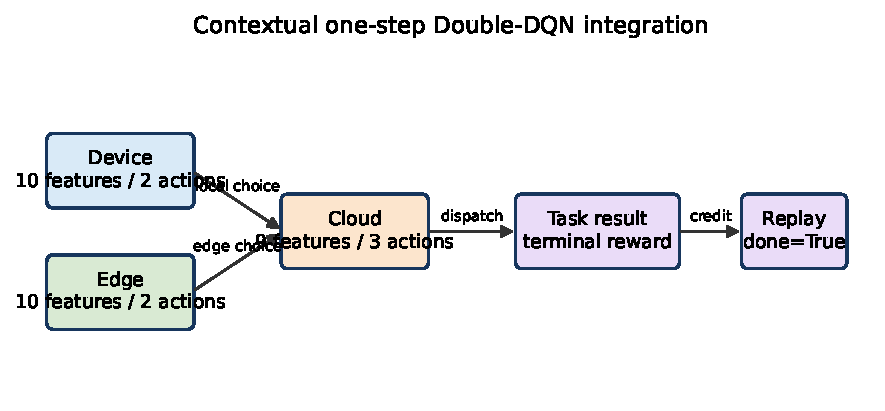
\includegraphics[width=\columnwidth]{figures/hierarchical_rl.pdf}
\caption{Local observations and terminal per-task credit.}
\label{fig:rl}
\end{figure}

\subsection{Coordination}
Feedback is adjacent-tier and causal: a message sampled at time $t$ becomes
available after propagation plus serialization at a later decision. Modes are
none, periodic, and frequent. Messages contribute recorded bytes and modeled
delay, but they do not contend with data-plane resources or block execution.
Thus the implementation measures control-plane accounting, not a complete
communication-latency trade-off. Fig.~\ref{fig:coordination} shows the
implemented information path.

\begin{figure}[t]
\centering
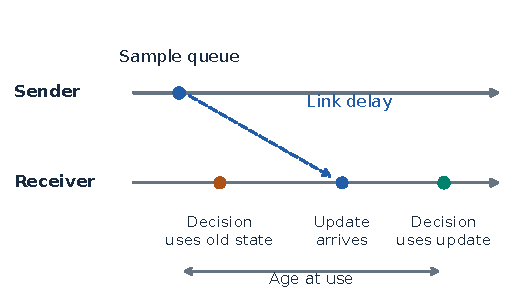
\includegraphics[width=\columnwidth]{figures/coordination.pdf}
\caption{Delayed adjacent-tier feedback; control traffic is non-blocking.}
\label{fig:coordination}
\end{figure}
